% ---------------------------------------------------------
% INTRODUCTION
% ---------------------------------------------------------
\section{Introduction}

This report presents the design and implementation of a 32-bit Single-Cycle RISC-V processor based on the RV32I instruction set. The architecture integrates essential hardware components, including an Arithmetic Logic Unit (ALU), Branch Comparison Unit (BRC), Register File, Immediate Generator, and a central Control Unit, all optimized to execute instructions within a single clock cycle. A specialized Load-Store Unit (LSU) is implemented to manage memory-mapped I/O, enabling the core to interface with external peripherals. The entire system is synthesized and deployed on the DE-2 FPGA development board. To demonstrate the functional integration of hardware and software, a practical application written in RISC-V Assembly is pre-loaded into the Instruction Memory (imem). This software allows the processor to interact with the board's physical components by reading input states from mechanical switches to control red LEDs and driving an LCD module for real-time status display.
% Viết giới thiệu tổng quan ở đây (như phần Lorem ipsum trong mẫu).
\newpage
% ---------------------------------------------------------
% DESIGN STRATEGY
% ---------------------------------------------------------
\section{Design Strategy}

\subsection{Overview}
% Tổng quan về kiến trúc Single-Cycle.
 \begin{figure}[h!]
	     \centering
	     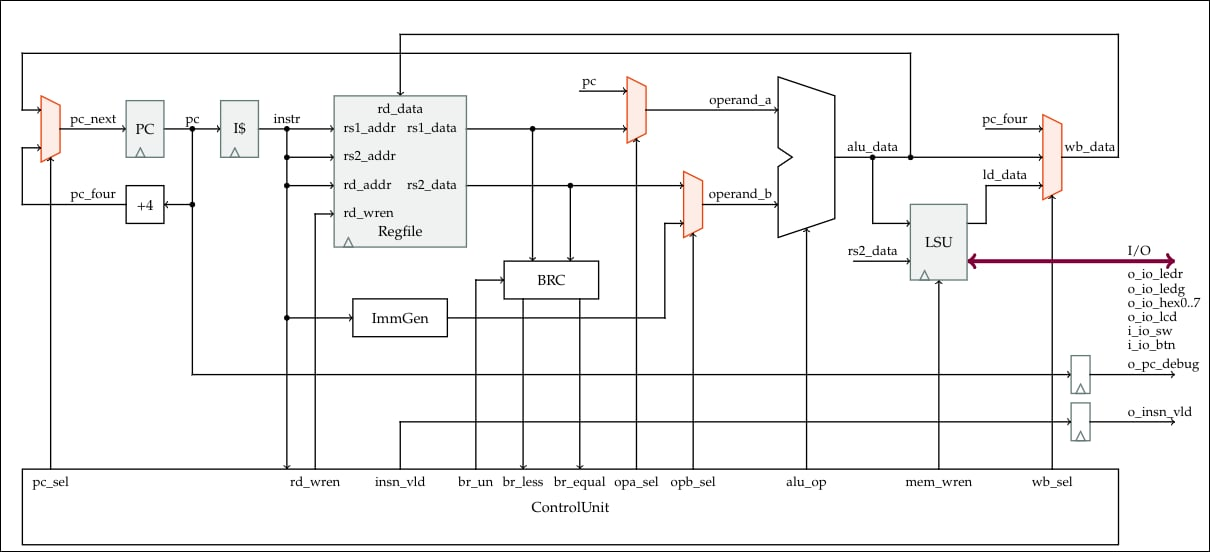
\includegraphics[width=1.0\linewidth]{figures_tech/single.jpg} 
	     \caption{Single Cycle Processor} % Thay bằng mô tả thực tế
	     \label{fig:sample_image} % Nhãn để tham chiếu
	 \end{figure}

The processor follows a single-cycle datapath architecture where each instruction is processed through several functional stages within one clock period. The cycle begins at the \textbf{Instruction Fetch} stage, where the Program Counter (PC) provides the address to the Instruction Memory ($I\$$) to retrieve the 32-bit instruction. Simultaneously, the PC value is incremented by 4 to prepare for the next sequential instruction.

In the \textbf{Instruction Decode} stage, the Control Unit interprets the opcode and function bits to generate synchronized control signals. The Register File (Regfile) reads data from source registers \texttt{rs1} and \texttt{rs2}, while the Immediate Generator (ImmGen) extracts and sign-extends immediate values according to the instruction format. For branch instructions, the Branch Comparison Unit (BRC) evaluates the relationship between operands to decide whether a branch should be taken.



The \textbf{Execute} stage utilizes the Arithmetic Logic Unit (ALU) to perform computations. The ALU operands are selected via multiplexers, allowing the core to process either register data or immediate values. The resulting \texttt{alu\_data} serves as the effective address for the \textbf{Load-Store Unit (LSU)}. The LSU acts as a bridge for memory-mapped I/O, managing access to the 2KiB data memory and interfacing with physical peripherals on the DE2 board, such as switches, LEDs, and the LCD. Finally, in the \textbf{Write-back} stage, a multiplexer selects between the ALU result, memory data, or the return address (\texttt{pc+4}) to update the destination register in the Regfile, completing the instruction execution.


\newpage
\subsection{ALU}
\begin{figure}[h!]
	
	\centering
	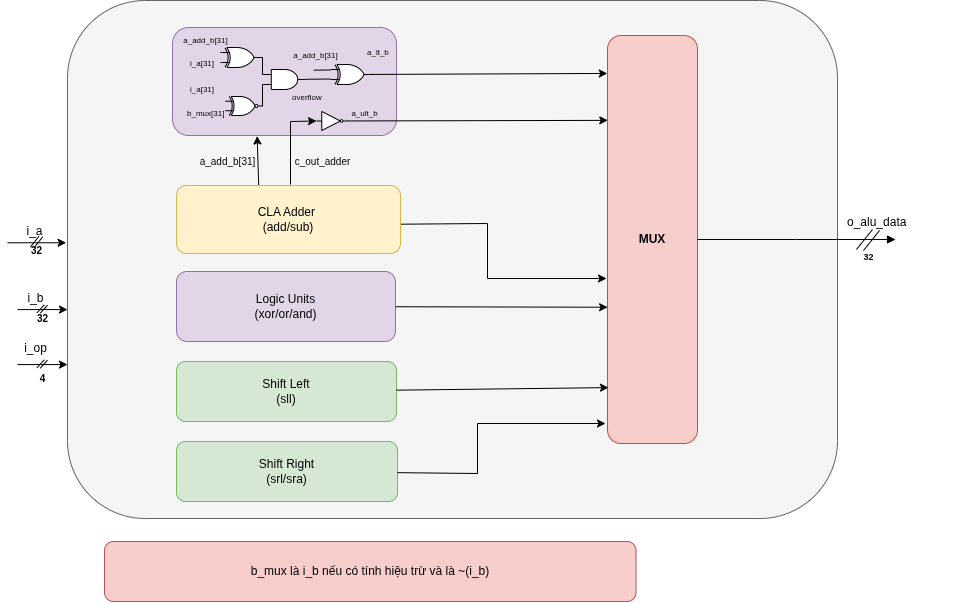
\includegraphics[width=1.0\linewidth]{figures_tech/alu111.png} 
	\caption{ALU} %
\end{figure}

% Mô tả khối ALU.
\subsubsection{Specification}
\begin{table}[h]
	\centering
	\begin{tabular}{l c c p{8cm}}
		\toprule
		\textbf{Signal} & \textbf{Width} & \textbf{Direction} & \textbf{Description} \\ \midrule
		\texttt{i\_a} & 32 & input & First operand for ALU operations. \\ 
		\texttt{i\_b} & 32 & input & Second operand for ALU operations. \\ 
		\texttt{i\_op} & 4 & input & Operation code selecting the specific arithmetic or logical function. \\ 
		\texttt{o\_alu\_data} & 32 & output & The 32-bit result of the ALU calculation. \\ 
		\texttt{o\_zero} & 1 & output & Zero flag; asserted to 1 if the result is 0, otherwise 0. \\ 
		\bottomrule
	\end{tabular}
	\caption{ALU Module Signal Description} % Chú thích nằm ở đây để hiển thị dưới bảng
	\label{tab:alu_spec}
\end{table}



\subsubsection{Implementation of Signed and Unsigned Comparisons}
A critical hardware optimization within this ALU design is the implementation of comparison operations (\texttt{SLT} and \texttt{SLTU}). Instead of instantiating dedicated hardware comparators, the datapath reuses the Carry-Lookahead Adder (\texttt{cla\_adder\_top}) to perform a subtraction ($A - B$). This is achieved by passing the 1's complement of operand B (\texttt{\textasciitilde B}) and setting the carry-in bit to 1. The comparison outcomes are then elegantly derived from the adder's status flags:

\begin{itemize}
	\item \textbf{Signed Comparison (\texttt{SLT}):} 
	Evaluating signed numbers requires careful handling of two's complement overflow. The overflow flag is asserted when operands of the same sign yield a sum of the opposite sign. The true "less than" mathematical condition is determined by XORing the sign bit of the result (\texttt{Sum[31]}) with the overflow flag:
	$$ \texttt{a\_lt\_b} = \texttt{Sum[31]} \oplus \texttt{overflow} $$
	This Boolean logic ensures that if a hardware overflow invalidates the apparent sign of the subtraction result, the XOR operation reverses it, always yielding the mathematically correct relationship.
	
	\item \textbf{Unsigned Comparison (\texttt{SLTU}):} 
	For unsigned numbers, the evaluation relies entirely on the carry-out (\texttt{c\_out\_adder}) of the 32-bit addition. When performing subtraction via two's complement ($A + \overline{B} + 1$), a carry-out of 0 explicitly indicates that a borrow occurred, meaning $A < B$. Conversely, a carry-out of 1 means $A \geq B$. Therefore, the unsigned "less than" condition is simply the inverted carry-out bit:
	$$ \texttt{a\_ult\_b} = \sim \texttt{c\_out\_adder} $$
\end{itemize}



\newpage
\subsection{BRC (Branch Comparison Unit)}

\begin{figure}[h!]
	
	\centering
	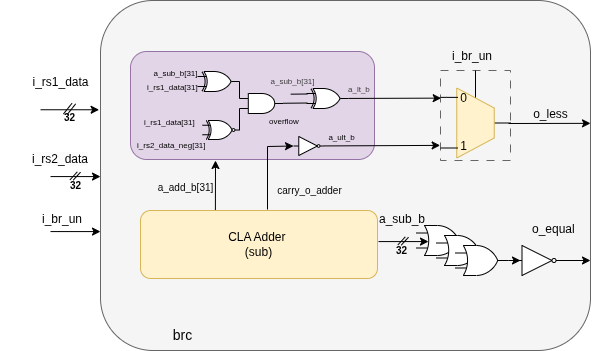
\includegraphics[width=1.0\linewidth]{figures_tech/brc111.png} 
	\caption{ALU} %
\end{figure}

% Mô tả khối BRC (trong spec gọi là BRC thay vì BRU).
\subsubsection{Specification}
\begin{table}[h]
	\centering
	\begin{tabular}{l c c p{8cm}}
		\toprule
		\textbf{Signal} & \textbf{Width} & \textbf{Direction} & \textbf{Description} \\ \midrule
		\texttt{i\_rs1\_data} & 32 & input & Data from the first source register. \\ 
		\texttt{i\_rs2\_data} & 32 & input & Data from the second source register. \\ 
		\texttt{i\_br\_un} & 1 & input & Unsigned comparison flag (1 for unsigned comparison, 0 for signed comparison). \\ 
		\texttt{o\_less} & 1 & output & Asserted to 1 if the first register is less than the second register. \\ 
		\texttt{o\_equal} & 1 & output & Asserted to 1 if the values of both registers are equal. \\ 
		\bottomrule
	\end{tabular}
	\caption{BRC Module Signal Description}
	\label{tab:brc_spec}
\end{table}

\subsubsection{Design}

The Branch Comparison Unit (BRC) is a dedicated hardware block designed to evaluate the conditional relationships between two source registers, providing immediate feedback to the Control Unit for branch decision-making. By analyzing the data from \texttt{rs1} and \texttt{rs2}, this unit determines whether a branch condition—such as equal, not equal, less than, or greater than—is satisfied.

To optimize hardware resources, the BRC reuses the high-speed Carry-Lookahead Adder (\texttt{cla\_adder\_top}) to perform a 32-bit subtraction ($A - B$). The status flags generated from this operation are used to derive the comparison results:
\begin{itemize}
	\item \textbf{Equality Logic:} The \texttt{o\_equal} signal is generated by performing a reduction NOR operation on the subtraction result. If all bits are zero, the operands are identical.
	\item \textbf{Signed Comparison:} The unit evaluates the "less than" condition for signed integers by XORing the result's sign bit with the overflow flag ($Sign \oplus Overflow$), ensuring mathematical correctness even when an overflow occurs.
	\item \textbf{Unsigned Comparison:} For unsigned operations, the unit monitors the carry-out bit. A lack of carry-out during subtraction indicates a borrow, signaling that the first operand is smaller than the second.
\end{itemize}
The final comparison outputs are multiplexed based on the \texttt{i\_br\_un} signal, allowing the processor to handle both signed and unsigned branch instructions accurately within a single cycle.
\newpage
\subsection{Regfile}

\begin{figure}[h!]
	
	\centering
	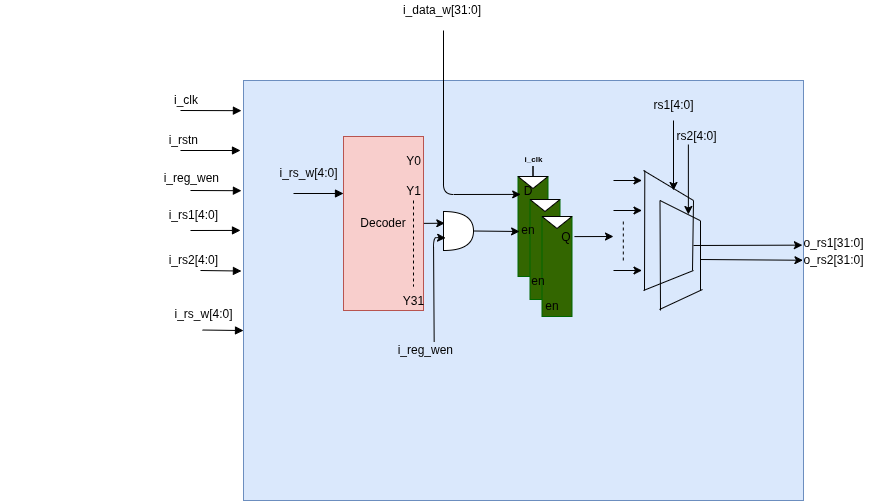
\includegraphics[width=1.0\linewidth]{figures_tech/reg_file.png} 
	\caption{Register File} %
\end{figure}


% Bổ sung theo Milestone 2: Mô tả tập thanh ghi 32x32-bit.
\subsubsection{Specification}
\begin{table}[h]
	\centering
	\begin{tabular}{l c c p{8cm}}
		\toprule
		\textbf{Signal} & \textbf{Width} & \textbf{Direction} & \textbf{Description} \\ \midrule
		\texttt{i\_clk} & 1 & input & Global clock signal. \\ 
		\texttt{i\_rstn} & 1 & input & Global active-low reset signal. \\ 
		\texttt{i\_reg\_wen} & 1 & input & Write enable signal (1 for write, 0 for read). \\ 
		\texttt{i\_rs1} & 5 & input & Address of the first source register. \\ 
		\texttt{i\_rs2} & 5 & input & Address of the second source register. \\ 
		\texttt{i\_rs\_w} & 5 & input & Address of the destination register. \\ 
		\texttt{i\_data\_w} & 32 & input & Data to write to the destination register. \\ 
		\texttt{o\_data\_1} & 32 & output & Data read from the first source register. \\ 
		\texttt{o\_data\_2} & 32 & output & Data read from the second source register. \\ 
		\bottomrule
	\end{tabular}
	\caption{Regfile Module Signal Description}
	\label{tab:regfile_spec}
\end{table}


The Register File (Regfile) serves as the primary high-speed storage for the processor, containing 32 general-purpose registers, each 32-bit wide. It is designed to handle simultaneous operations through two asynchronous read ports and one synchronous write port.


\begin{itemize}
	\item \textbf{Storage Capacity:} A total of 32 registers (x0 to x31), providing operands for the ALU and storing calculation results.
	\item \textbf{Register x0 Constraint:} In strict adherence to the RISC-V ISA, register 0 is hardwired to zero. The logic ensures that any write operations to address \texttt{5'b00000} are ignored, while read operations from this address always return \texttt{32'b0}.
	\item \textbf{Access Logic:} Data is read asynchronously to allow the datapath to process information immediately within the clock cycle, while writing occurs on the rising edge of the global clock when the write enable (\texttt{i\_reg\_wen}) is asserted.
\end{itemize}
\newpage
\subsection{IMEM}
% Bổ sung theo Milestone 2: Mô tả bộ nhớ lệnh và dữ liệu.
\subsubsection{Specification}
\begin{table}[h]
	\centering
	\begin{tabular}{l c c p{8cm}}
		\toprule
		\textbf{Signal} & \textbf{Width} & \textbf{Direction} & \textbf{Description} \\ \midrule
		\texttt{i\_pc\_addr} & 30 & input & Word-aligned instruction address derived from the Program Counter (PC[31:2]). \\ 
		\texttt{o\_inst} & 32 & output & The 32-bit instruction fetched from the memory array. \\ 
		\bottomrule
	\end{tabular}
	\caption{Instruction Memory Module Signal Description}
	\label{tab:imem_spec}
\end{table}
The Instruction Memory (imem) is a 2KiB read-only memory module designed to store and provide machine code during the fetch stage. It utilizes a 30-bit word-aligned address derived from the Program Counter to asynchronously retrieve 32-bit instructions from an array of 2048 entries. The implementation uses the lower 11 bits of the address for indexing and is initialized via the \texttt{\$readmemh} system task, ensuring that the required instruction is available to the datapath immediately within a single clock cycle without any timing latency.


\newpage


\subsection{LSU (Load-Store Unit)}

\begin{figure}[H]
	
	\centering
	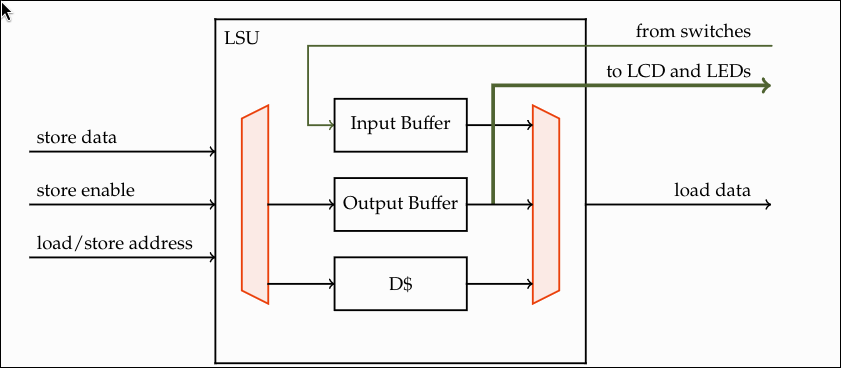
\includegraphics[width=1.0\linewidth]{figures_tech/lsu.png} 
	\caption{LSU} %
\end{figure}


% Bổ sung theo Milestone 2: Mô tả khối Load-Store Unit và Memory Mapping.
\subsubsection{Specification}
\begin{table}[h]
	\centering
	\begin{tabular}{l c c p{7.5cm}}
		\toprule
		\textbf{Signal} & \textbf{Width} & \textbf{Direction} & \textbf{Description} \\ \midrule
		\texttt{i\_clk} & 1 & input & Global clock, active on the rising edge. \\ 
		\texttt{i\_reset} & 1 & input & Global active reset. \\ 
		\texttt{i\_funct3} & 3 & input & Specifies data size (byte, half-word, word) and sign-extension. \\ 
		\texttt{i\_lsu\_addr} & 32 & input & Address for data read/write operations. \\ 
		\texttt{i\_st\_data} & 32 & input & Data to be stored into memory or peripherals. \\ 
		\texttt{i\_lsu\_wren} & 1 & input & Write enable signal (1 for write, 0 for read). \\ 
		\texttt{o\_ld\_data} & 32 & output & Data loaded from memory or switch inputs. \\ 
		\texttt{o\_io\_ledr} & 32 & output & Output driving the red LEDs. \\ 
		\texttt{o\_io\_ledg} & 32 & output & Output driving the green LEDs. \\ 
		\texttt{o\_io\_hex0..7} & 7 & output & Outputs driving the eight 7-segment displays. \\ 
		\texttt{o\_io\_lcd} & 32 & output & Output driving the LCD control registers. \\ 
		\texttt{i\_io\_sw} & 32 & input & Input from the physical hardware switches. \\ 
		\bottomrule
	\end{tabular}
	\caption{LSU Module Signal Description}
	\label{tab:lsu_spec}
\end{table}
\newpage
\section{Memory and I/O System Implementation}
\subsection{Address Decoding and Memory Mapping}
The Load-Store Unit (LSU) manages the communication between the processor and various memory-mapped components by decoding the 32-bit address bus (\texttt{i\_lsu\_addr}). The decoding logic specifically checks the upper 20 bits (\texttt{i\_lsu\_addr[31:12]}) to determine the target device and set the corresponding activation flags. According to the system specification, the memory space is partitioned as follows:
\begin{itemize}
	\item \textbf{Data Memory (2KiB RAM):} Mapped to the range \texttt{0x0000\_0000} to \texttt{0x0000\_07FF}. The LSU activates the \texttt{dmem\_flag} when the upper bits are \texttt{20'h00000} and bit 11 is 0.
	\item \textbf{Output Peripherals:} Specific address ranges activate dedicated flags for the Red LEDs (\texttt{20'h10000}), Green LEDs (\texttt{20'h10001}), Seven-segment displays (\texttt{20'h10002} for HEX0-3 and \texttt{20'h10003} for HEX4-7), and the LCD Control Registers (\texttt{20'h10004}).
	\item \textbf{Input Peripherals:} The Switches are mapped to the address range starting at \texttt{0x1001\_0000} (\texttt{20'h10010}), which triggers the \texttt{switch\_flag}.
\end{itemize}

\subsection{Data Memory Access Mechanism}
The Data Memory (\texttt{dmem}) module is designed with synchronous write and asynchronous read capabilities.
\begin{itemize}
	\item \textbf{Store Operations:} When a store instruction is executed, the LSU aligns the data (\texttt{st\_data\_aligned}) based on the instruction type (Byte, Half-word, or Word). A 4-bit byte mask (\texttt{i\_bmask}) is generated using the lower address bits (\texttt{i\_lsu\_addr[1:0]}) to selectively write only the target bytes into the memory array during the rising clock edge.
	\item \textbf{Load Operations:} For load instructions, data is asynchronously retrieved from the memory or peripheral buffer. The LSU then performs right-alignment and sign-extension (for \texttt{LB}, \texttt{LH}) or zero-extension (for \texttt{LBU}, \texttt{LHU}) based on the \texttt{i\_funct3} field to provide the final 32-bit data to the processor.
\end{itemize}
\newpage
\subsection{Peripheral I/O Interface Control}
The system utilizes dedicated buffer modules to interface with hardware components through the Memory-Mapped I/O (MMIO) scheme.
\begin{itemize}
	\item \textbf{Output Buffering:} The \texttt{output\_buffer} module latches data for external displays and indicators. It updates the state of LEDs, HEX displays, or the LCD registers only when the respective peripheral flag and the global write enable (\texttt{i\_lsu\_wren}) are active, while adhering to the byte-masking requirements.
	\item \textbf{Input Buffering:} The \texttt{input\_buffer} module gates the 32-bit physical switch data (\texttt{i\_io\_sw}) onto the internal data bus only when the \texttt{switch\_flag} is active. This ensures that the processor reads valid hardware status only when accessing the designated switch address space.
\end{itemize}


\newpage
\subsection{Immediate Generator}
% The Immediate Generator extracts and sign-extends the immediate values based on the instruction format (I, S, B, U, J).

\subsubsection{Specification}
\begin{table}[h]
	\centering
	\begin{tabular}{l c c p{7.5cm}}
		\toprule
		\textbf{Signal} & \textbf{Width} & \textbf{Direction} & \textbf{Description} \\ \midrule
		\texttt{i\_inst} & 32 & input & The 32-bit instruction fetched from Instruction Memory. \\ 
		\texttt{i\_imm\_sel} & 3 & input & Immediate format selector (I, S, B, U, J type) from the Control Unit. \\ 
		\texttt{o\_imm} & 32 & output & The 32-bit sign-extended immediate value. \\ 
		\bottomrule
	\end{tabular}
	\caption{Immediate Generator Signal Description}
	\label{tab:imm_gen_spec}
\end{table}

The Immediate Generator (ImmGen) is a combinational logic block responsible for extracting and sign-extending immediate values from the 32-bit instruction. Depending on the instruction format—specifically I, S, B, U, or J types—the unit rearranges the appropriate bit fields and extends the most significant bit (sign bit) to produce a complete 32-bit immediate operand. This extraction process is dynamically controlled by the \texttt{i\_imm\_sel} signal from the Control Unit, ensuring that the correctly formatted constant is available for the ALU or branch address calculation without any clock cycle latency.
% ---------------------------------------------------------
\newpage

\subsection{Control Unit}

\begin{figure}[H]
	
	\centering
	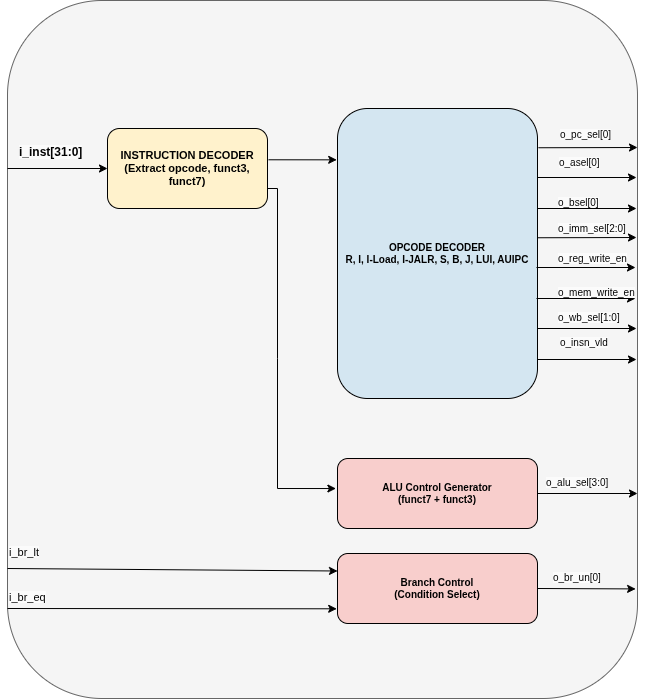
\includegraphics[width=1.0\linewidth]{figures_tech/ctrl.png} 
	\caption{Control Logic} %
\end{figure}

% The Control Unit decodes the 32-bit instruction to generate control signals for the datapath.
\newpage
\subsubsection{Specification}
\begin{table}[h]
	\centering
	\begin{tabular}{l c c p{7.5cm}}
		\toprule
		\textbf{Signal} & \textbf{Width} & \textbf{Direction} & \textbf{Description} \\ \midrule
		\texttt{i\_inst} & 32 & input & The 32-bit instruction fetched from Instruction Memory. \\ 
		\texttt{i\_br\_lt} & 1 & input & Less-than flag from the Branch Comparison Unit (BRC). \\ 
		\texttt{i\_br\_eq} & 1 & input & Equal flag from the Branch Comparison Unit (BRC). \\ 
		\texttt{o\_pc\_sel} & 1 & output & PC source selector (0: PC+4, 1: ALU Result for branch/jump). \\ 
		\texttt{o\_imm\_sel} & 3 & output & Immediate format selector (I, S, B, U, J type). \\ 
		\texttt{o\_br\_un} & 1 & output & Branch unsigned flag (1 for unsigned, 0 for signed comparison). \\ 
		\texttt{o\_asel} & 1 & output & ALU operand A selector (0: \texttt{rs1}, 1: PC). \\ 
		\texttt{o\_bsel} & 1 & output & ALU operand B selector (0: \texttt{rs2}, 1: Immediate). \\ 
		\texttt{o\_reg\_write\_en} & 1 & output & Register file write enable signal. \\ 
		\texttt{o\_alu\_sel} & 4 & output & ALU operation selector code. \\ 
		\texttt{o\_mem\_write\_en} & 1 & output & Data memory write enable signal. \\ 
		\texttt{o\_wb\_sel} & 2 & output & Write-back data selector (00: Memory, 01: ALU, 10: PC+4). \\ 
		\texttt{o\_insn\_vld} & 1 & output & Instruction valid flag (1 if the instruction is supported, 0 otherwise). \\ 
		\bottomrule
	\end{tabular}
	\caption{Control Unit Signal Description}
	\label{tab:control_unit_spec}
\end{table}


\begin{figure}[h!]
	\caption{Decode For Control Logic} % Thay bằng mô tả thực tế
	\centering
	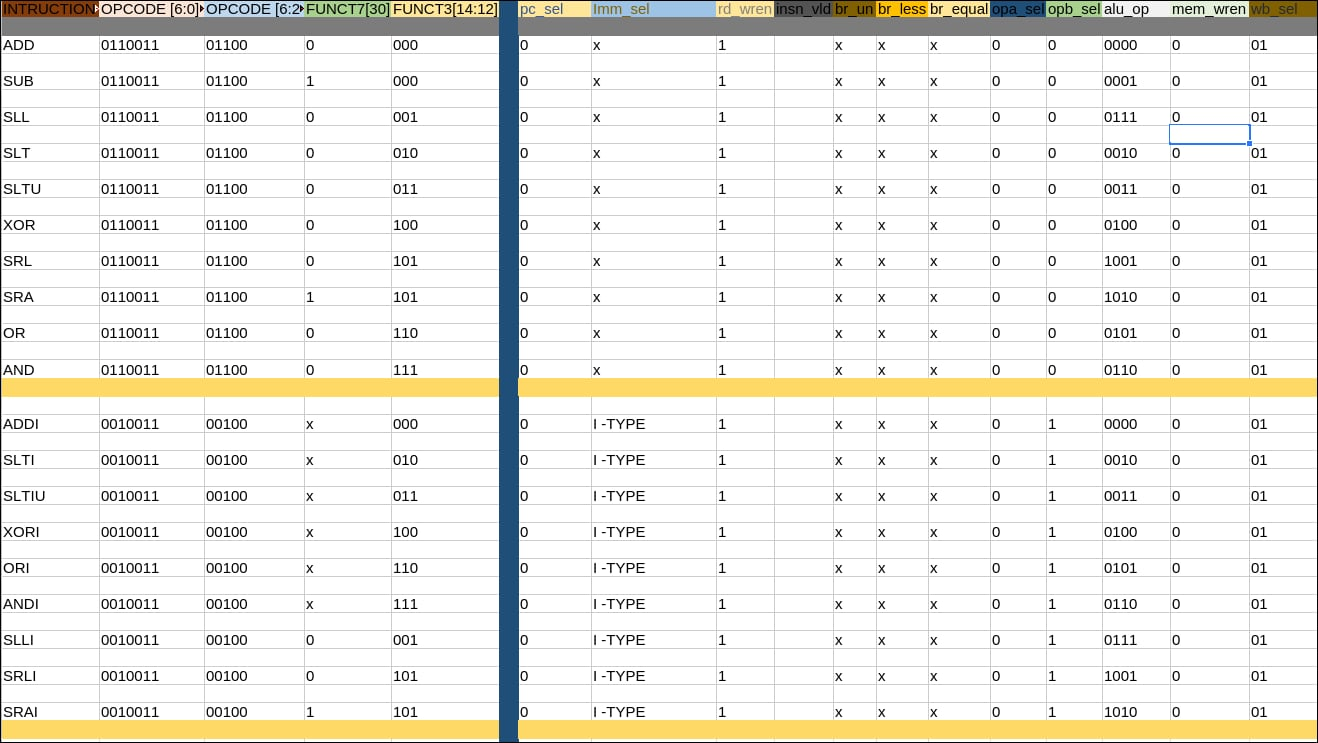
\includegraphics[width=1.0\linewidth]{figures_tech/c1.jpg} 
	
\end{figure}


\begin{figure}[h!]
	\centering
	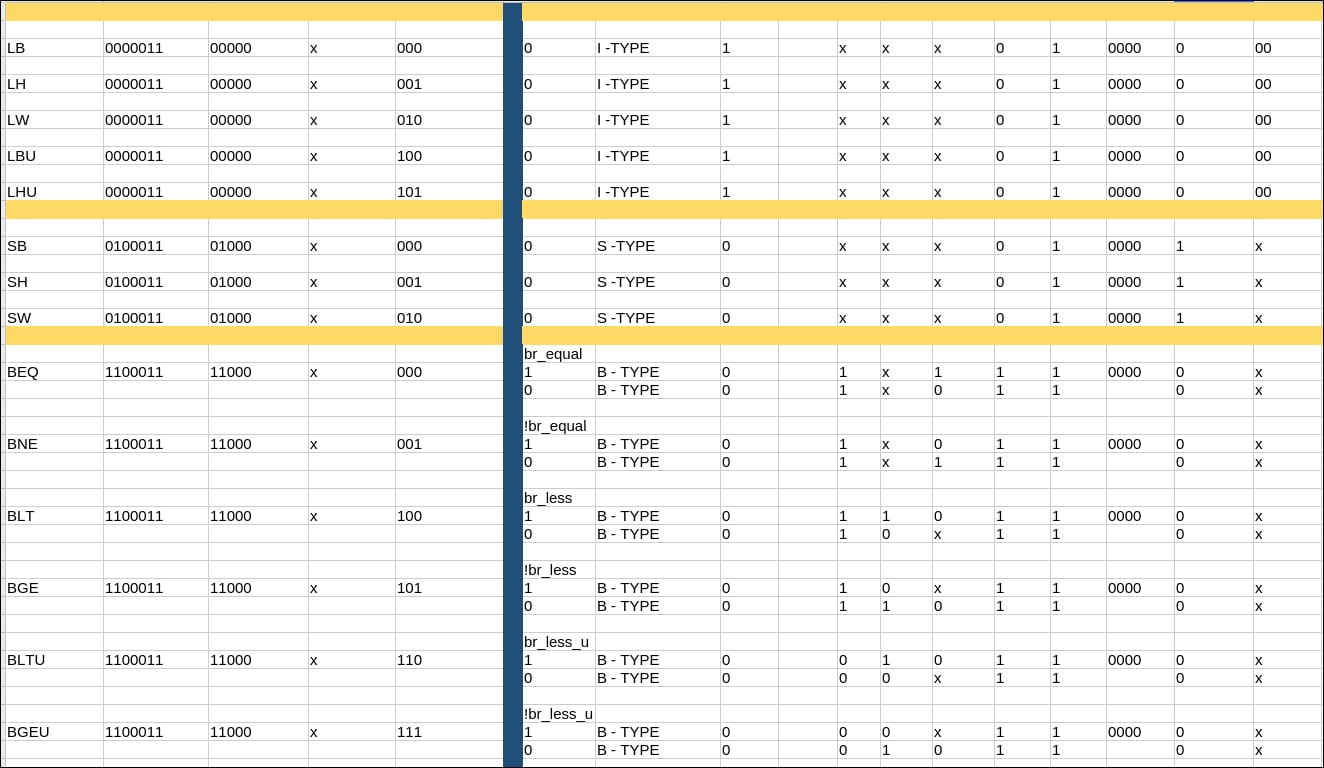
\includegraphics[width=1.0\linewidth]{figures_tech/c2.jpg} 

\end{figure}

\begin{figure}[h!]
	\centering
	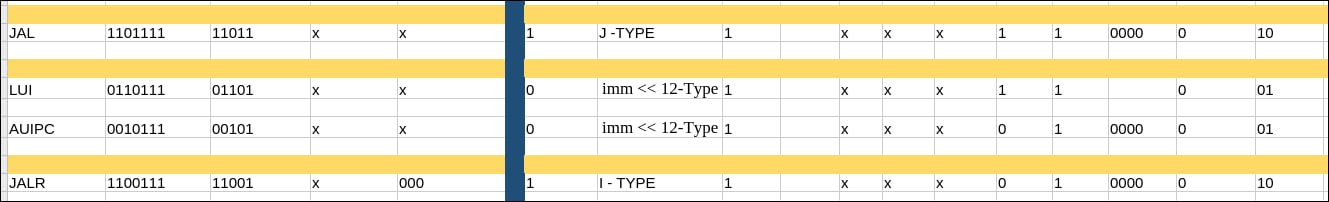
\includegraphics[width=1.0\linewidth]{figures_tech/c3.jpg} 

\end{figure}

\newpage






% ---------------------------------------------------------
% VERIFICATION STRATEGY
% ---------------------------------------------------------
\newpage
\section{Server Simulation Results }
% Cấu trúc phần này giữ nguyên theo file docx mẫu.

\begin{figure}[H]
	\centering
	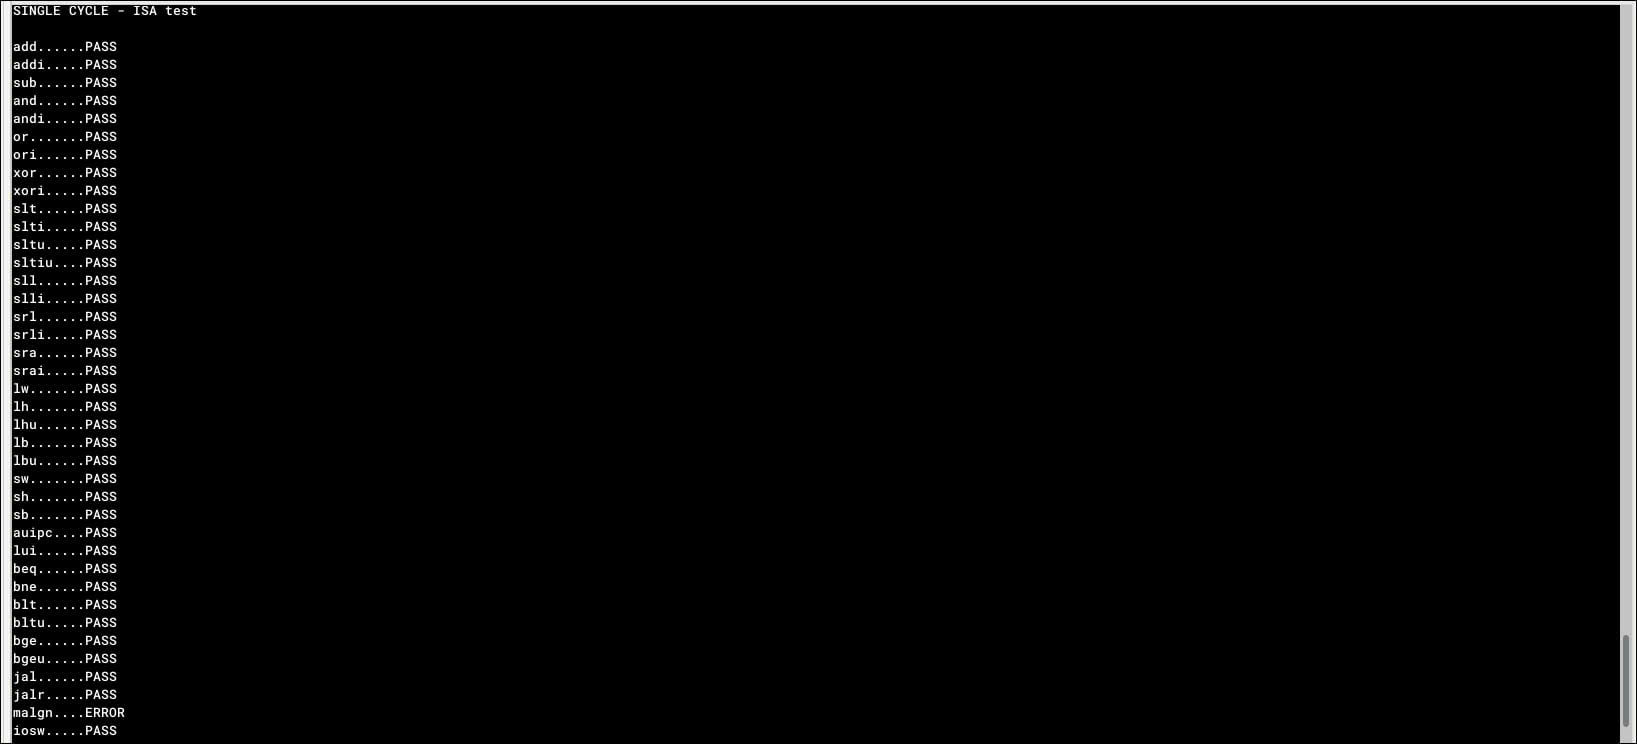
\includegraphics[width=1.0\linewidth]{figures_tech/pass.jpg} 
	\caption{Simulation Log}
\end{figure}
\newpage


\section{FPGA DE2 Implementation}
\subsection{Application: Single LED Control via Switch (SW to LEDR)}

\begin{figure}[H]
	\centering
	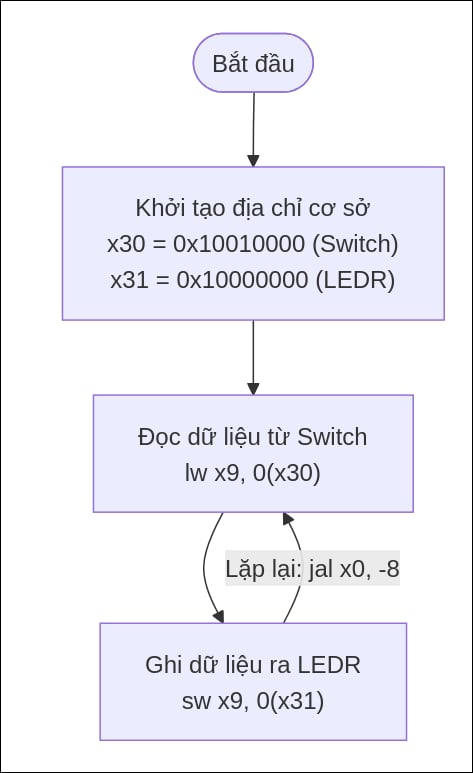
\includegraphics[width=0.7\linewidth]{figures_tech/sw_ledr.jpg} 
	\caption{Drive Switch To LEDR}
\end{figure}

\begin{figure}[H]
	\centering
	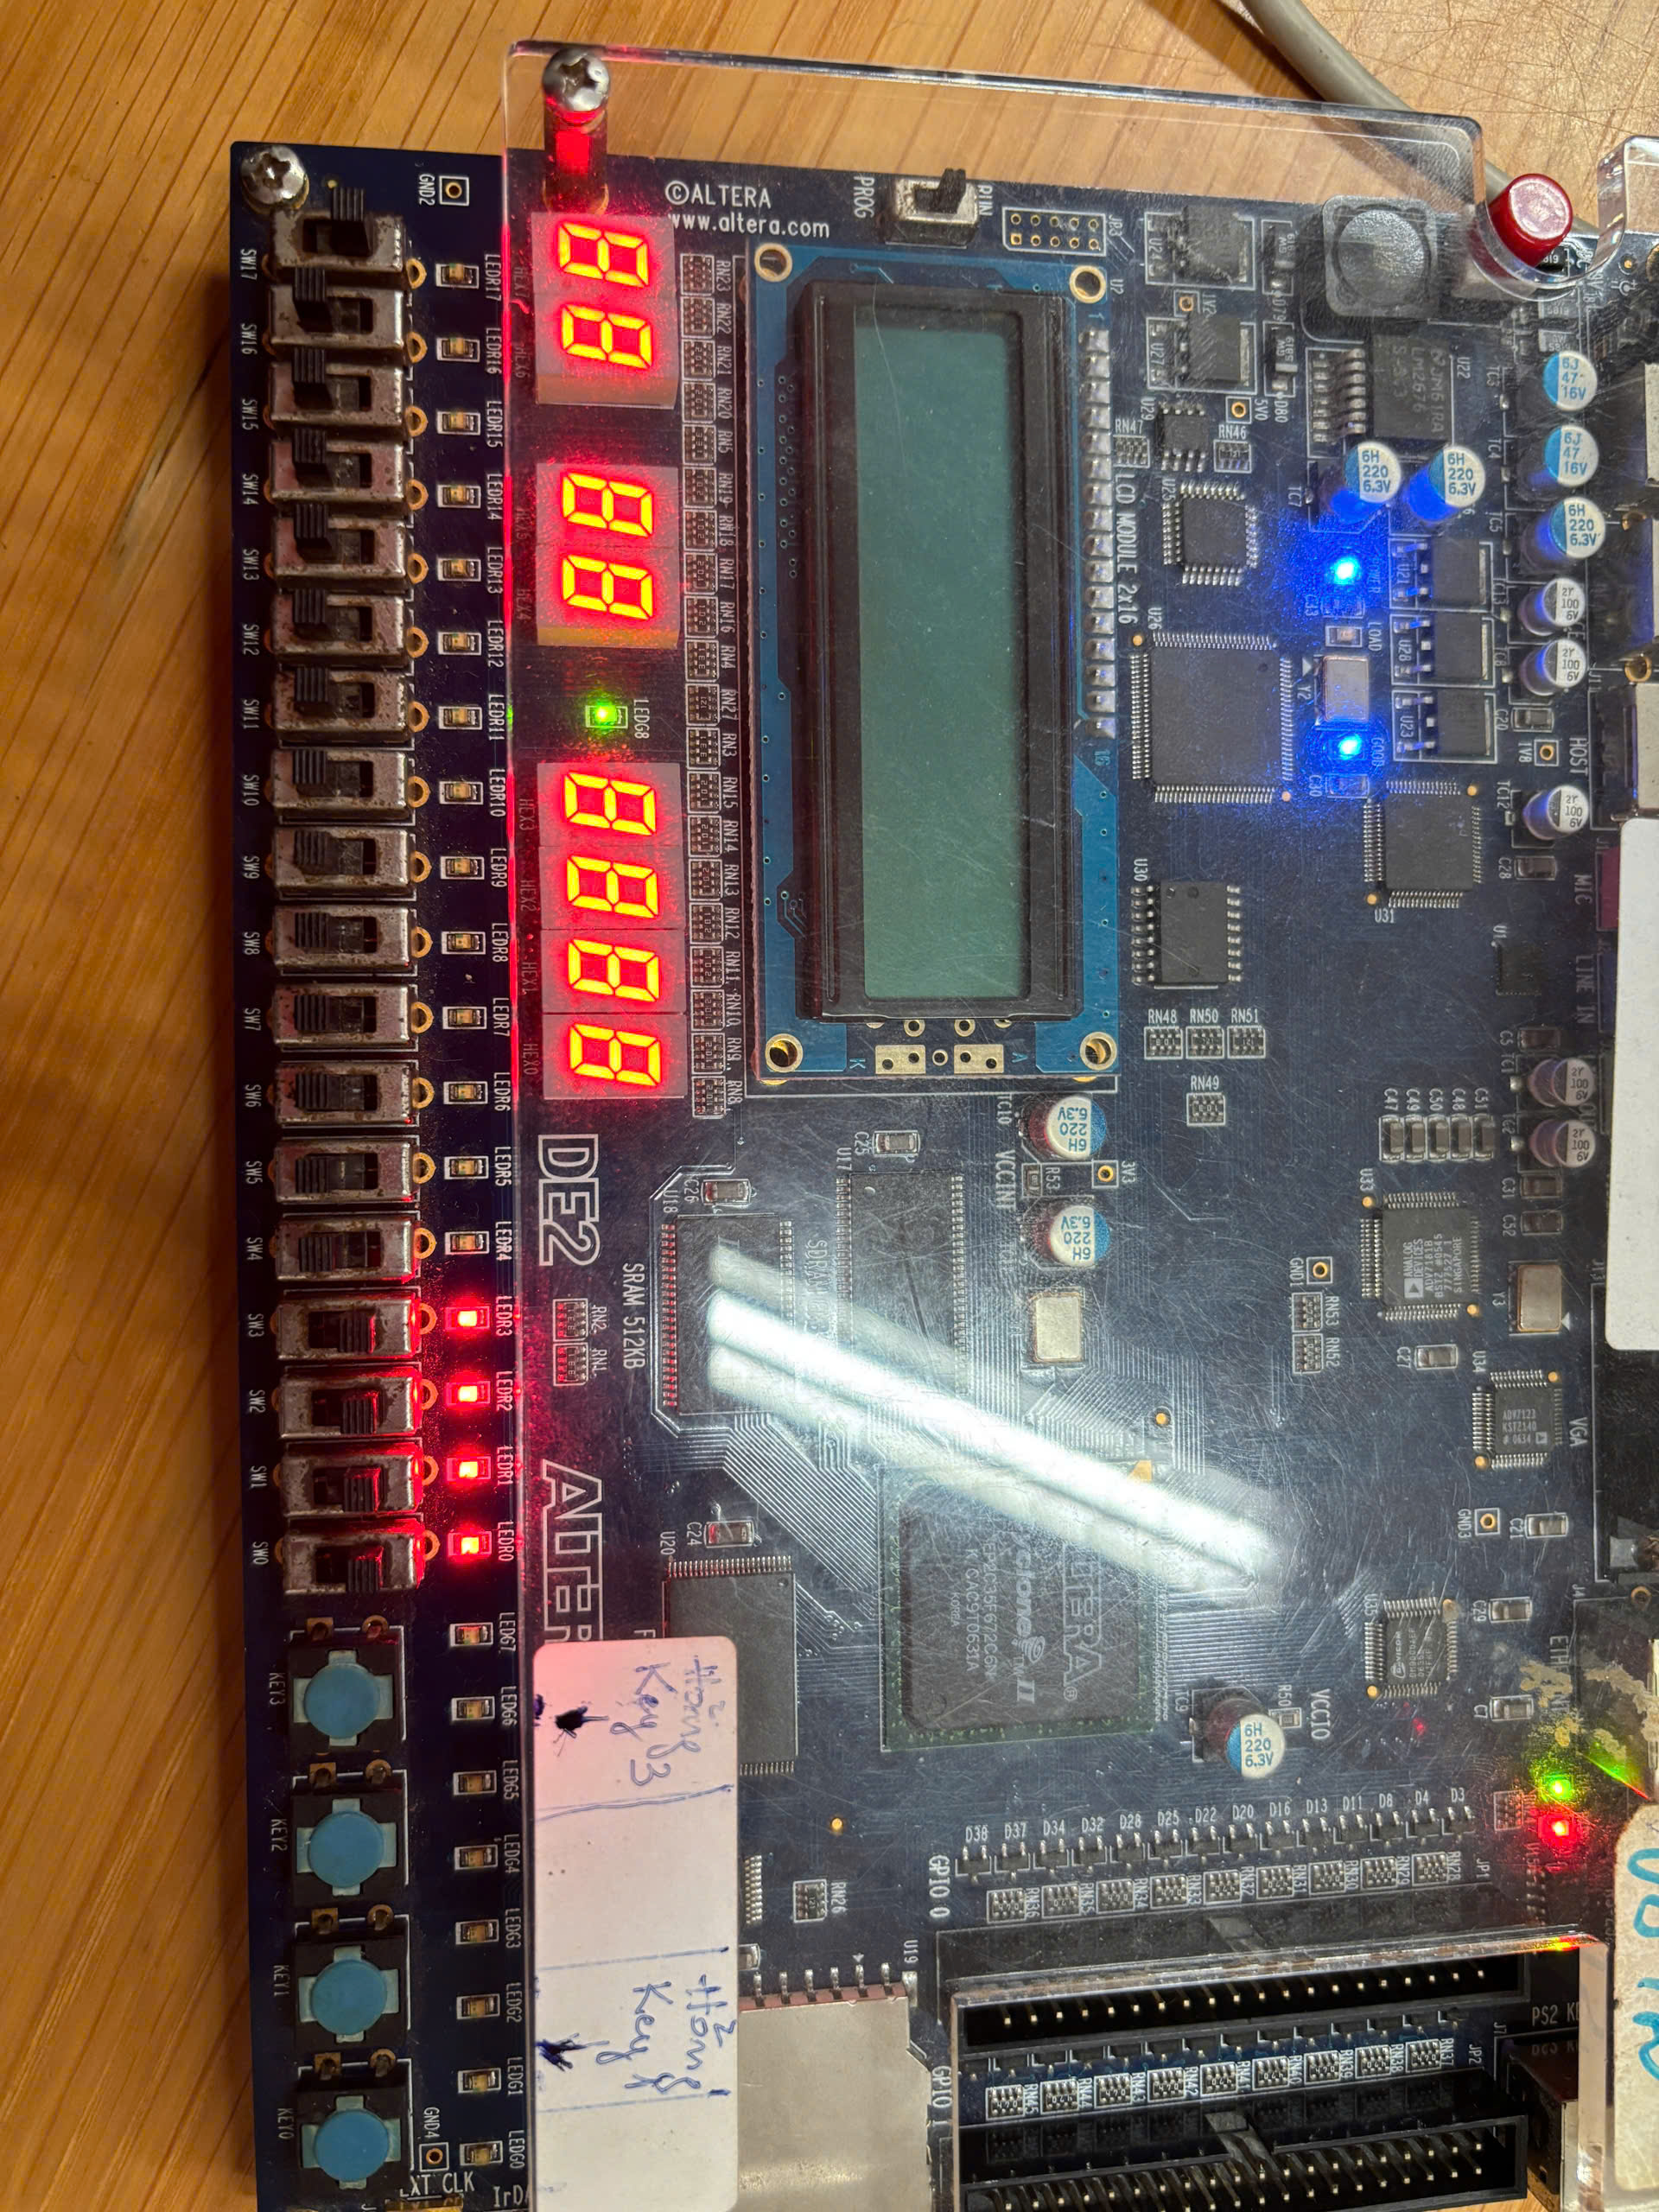
\includegraphics[width=0.7\linewidth]{figures_tech/sw_2_ledr.jpg} 
	\caption{Drive Switch To LEDR}
\end{figure}

\newpage
The algorithm of this application focuses on establishing a direct data flow between the input device (Switch) and the output device (Red LED) through the technique of Memory-Mapped I/O. The operation process is described in the following steps:

\begin{enumerate}
	\item \textbf{Memory Initialization:} The algorithm begins by loading the base addresses of the peripherals into the processor registers using the \texttt{lui} instruction. According to the LSU memory mapping, the Switch cluster is mapped at the base address \texttt{0x10010000} (loaded into register \texttt{x30}), and the Red LED cluster (LEDR) is mapped at \texttt{0x10000000} (loaded into register \texttt{x31}).
	\item \textbf{Continuous Polling Loop:} The CPU enters an infinite loop (marked by the \texttt{loop} label), continuously executing the load word instruction (\texttt{lw}) from the Switch base address (\texttt{x30}) and saving it into a temporary register (\texttt{x9}). The retrieved data is a bit string representing the current logic levels (On/Off) of the physical switches on the FPGA board.
	\item \textbf{State Update:} The data just read into \texttt{x9} is immediately written (\texttt{sw}) to the memory address of the LEDR (\texttt{x31}). Finally, an unconditional jump (\texttt{jal x0, -8}) forces the program counter back by 8 bytes (equivalent to 2 instructions) to repeat the loop. This high-speed repetitive operation ensures that the LEDs respond in real time whenever the user changes the state of the Switch.
\end{enumerate}



\newpage
\subsection{Application: Displaying Switch Value on 7-Segment LED (SW to HEX)}
\begin{figure}[H]
	\centering
	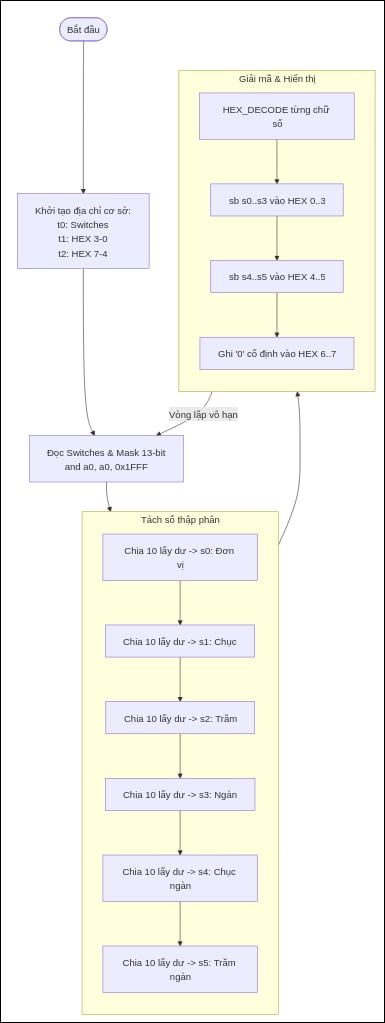
\includegraphics[width=0.5\linewidth]{figures_tech/swhex.jpg} 
	\caption{Drive Switch To HEX}
\end{figure}

\begin{figure}[H]
	\centering
	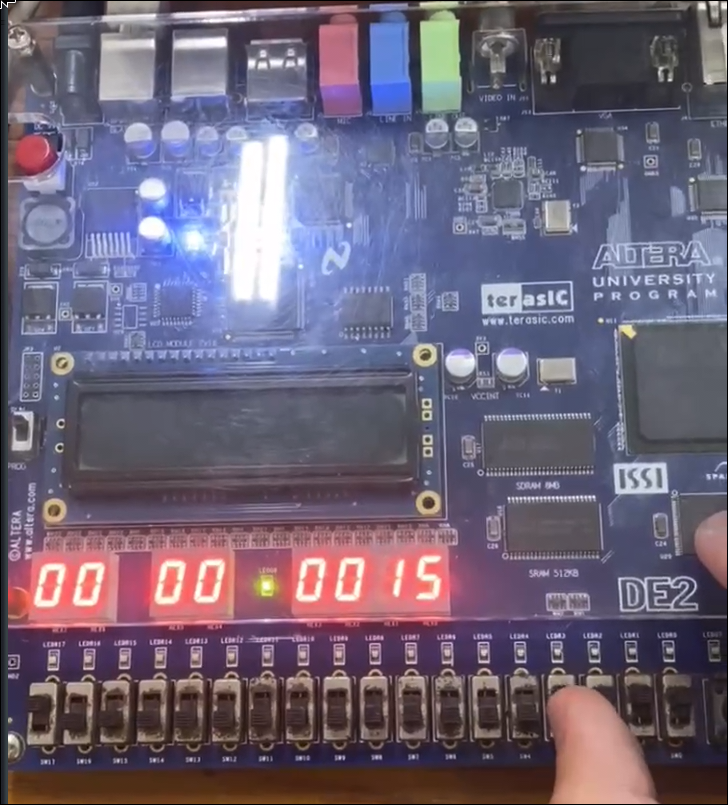
\includegraphics[width=0.7\linewidth]{figures_tech/SW_to_HEX.png} 
	\caption{Drive Switch To HEX (1111 -> 15)}
\end{figure}

Unlike direct data transfer, this application requires a more complex algorithm to convert raw binary data into decimal numbers that can be displayed on the 7-segment LED system. The algorithm includes the following core processing blocks:

\begin{enumerate}
	\item \textbf{Data Reading and Masking:} The system initializes the I/O base addresses for the Switches (\texttt{0x10010000}) and two HEX display clusters: HEX 3-0 (\texttt{0x10002000}) and HEX 7-4 (\texttt{0x10003000}). Raw data from the Switches is read into register \texttt{a0}, then an \texttt{and} operation with a 13-bit mask (\texttt{0x1FFF}) is performed to limit the input value to a maximum of 8191.
	\item \textbf{Decimal Digit Extraction:} The filtered value is processed through the \texttt{DIV10\_MOD10} subroutine. By repeatedly dividing by 10 and taking the remainder, the algorithm extracts six individual decimal digits (from units to hundred-thousands), storing them in registers \texttt{s0} through \texttt{s5}.
	\item \textbf{Decoding:} Each extracted digit is passed into the \texttt{HEX\_DECODE} subroutine. This block uses a branching structure (\texttt{beq}) to map numeric values (0–9) to their corresponding 7-segment active-low control codes (e.g., \texttt{0x40} for digit '0', \texttt{0x79} for digit '1', and \texttt{0x10} for digit '9').
	\item \textbf{Display Output:} The decoded codes are written to the peripheral memory using the Store Byte (\texttt{sb}) instruction. The first four digits (\texttt{s0-s3}) are sent to offsets \texttt{0, 1, 2, 3} of the first cluster (\texttt{t1}), while the remaining two digits (\texttt{s4-s5}) are sent to offsets \texttt{0, 1} of the second cluster (\texttt{t2}).
	\item \textbf{Display Formatting:} To ensure a consistent 8-digit display, the algorithm manually writes the code \texttt{0x40} (representing digit '0') to the two highest positions (HEX6 and HEX7) at offsets \texttt{2} and \texttt{3} of the second cluster (\texttt{t2}).
\end{enumerate}

\newpage
\subsection{Application: Stopwatch on 7-Segment LEDs}

\begin{figure}[H]
	\centering
	% Thay đổi đường dẫn ảnh thực tế của bạn tại đây
	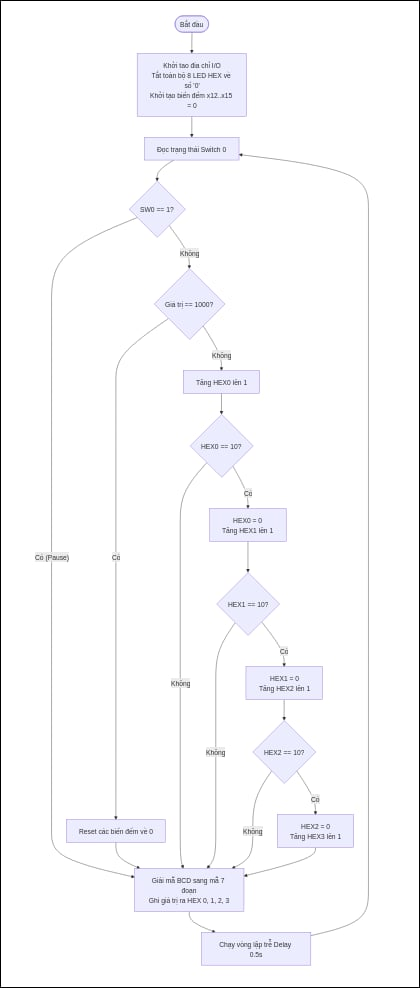
\includegraphics[width=0.5\linewidth]{figures_tech/stw.jpg} 
	\caption{Stopwatch Application Running}
\end{figure}

\begin{figure}[H]
	\centering
	% Thay đổi đường dẫn ảnh thực tế của bạn tại đây
	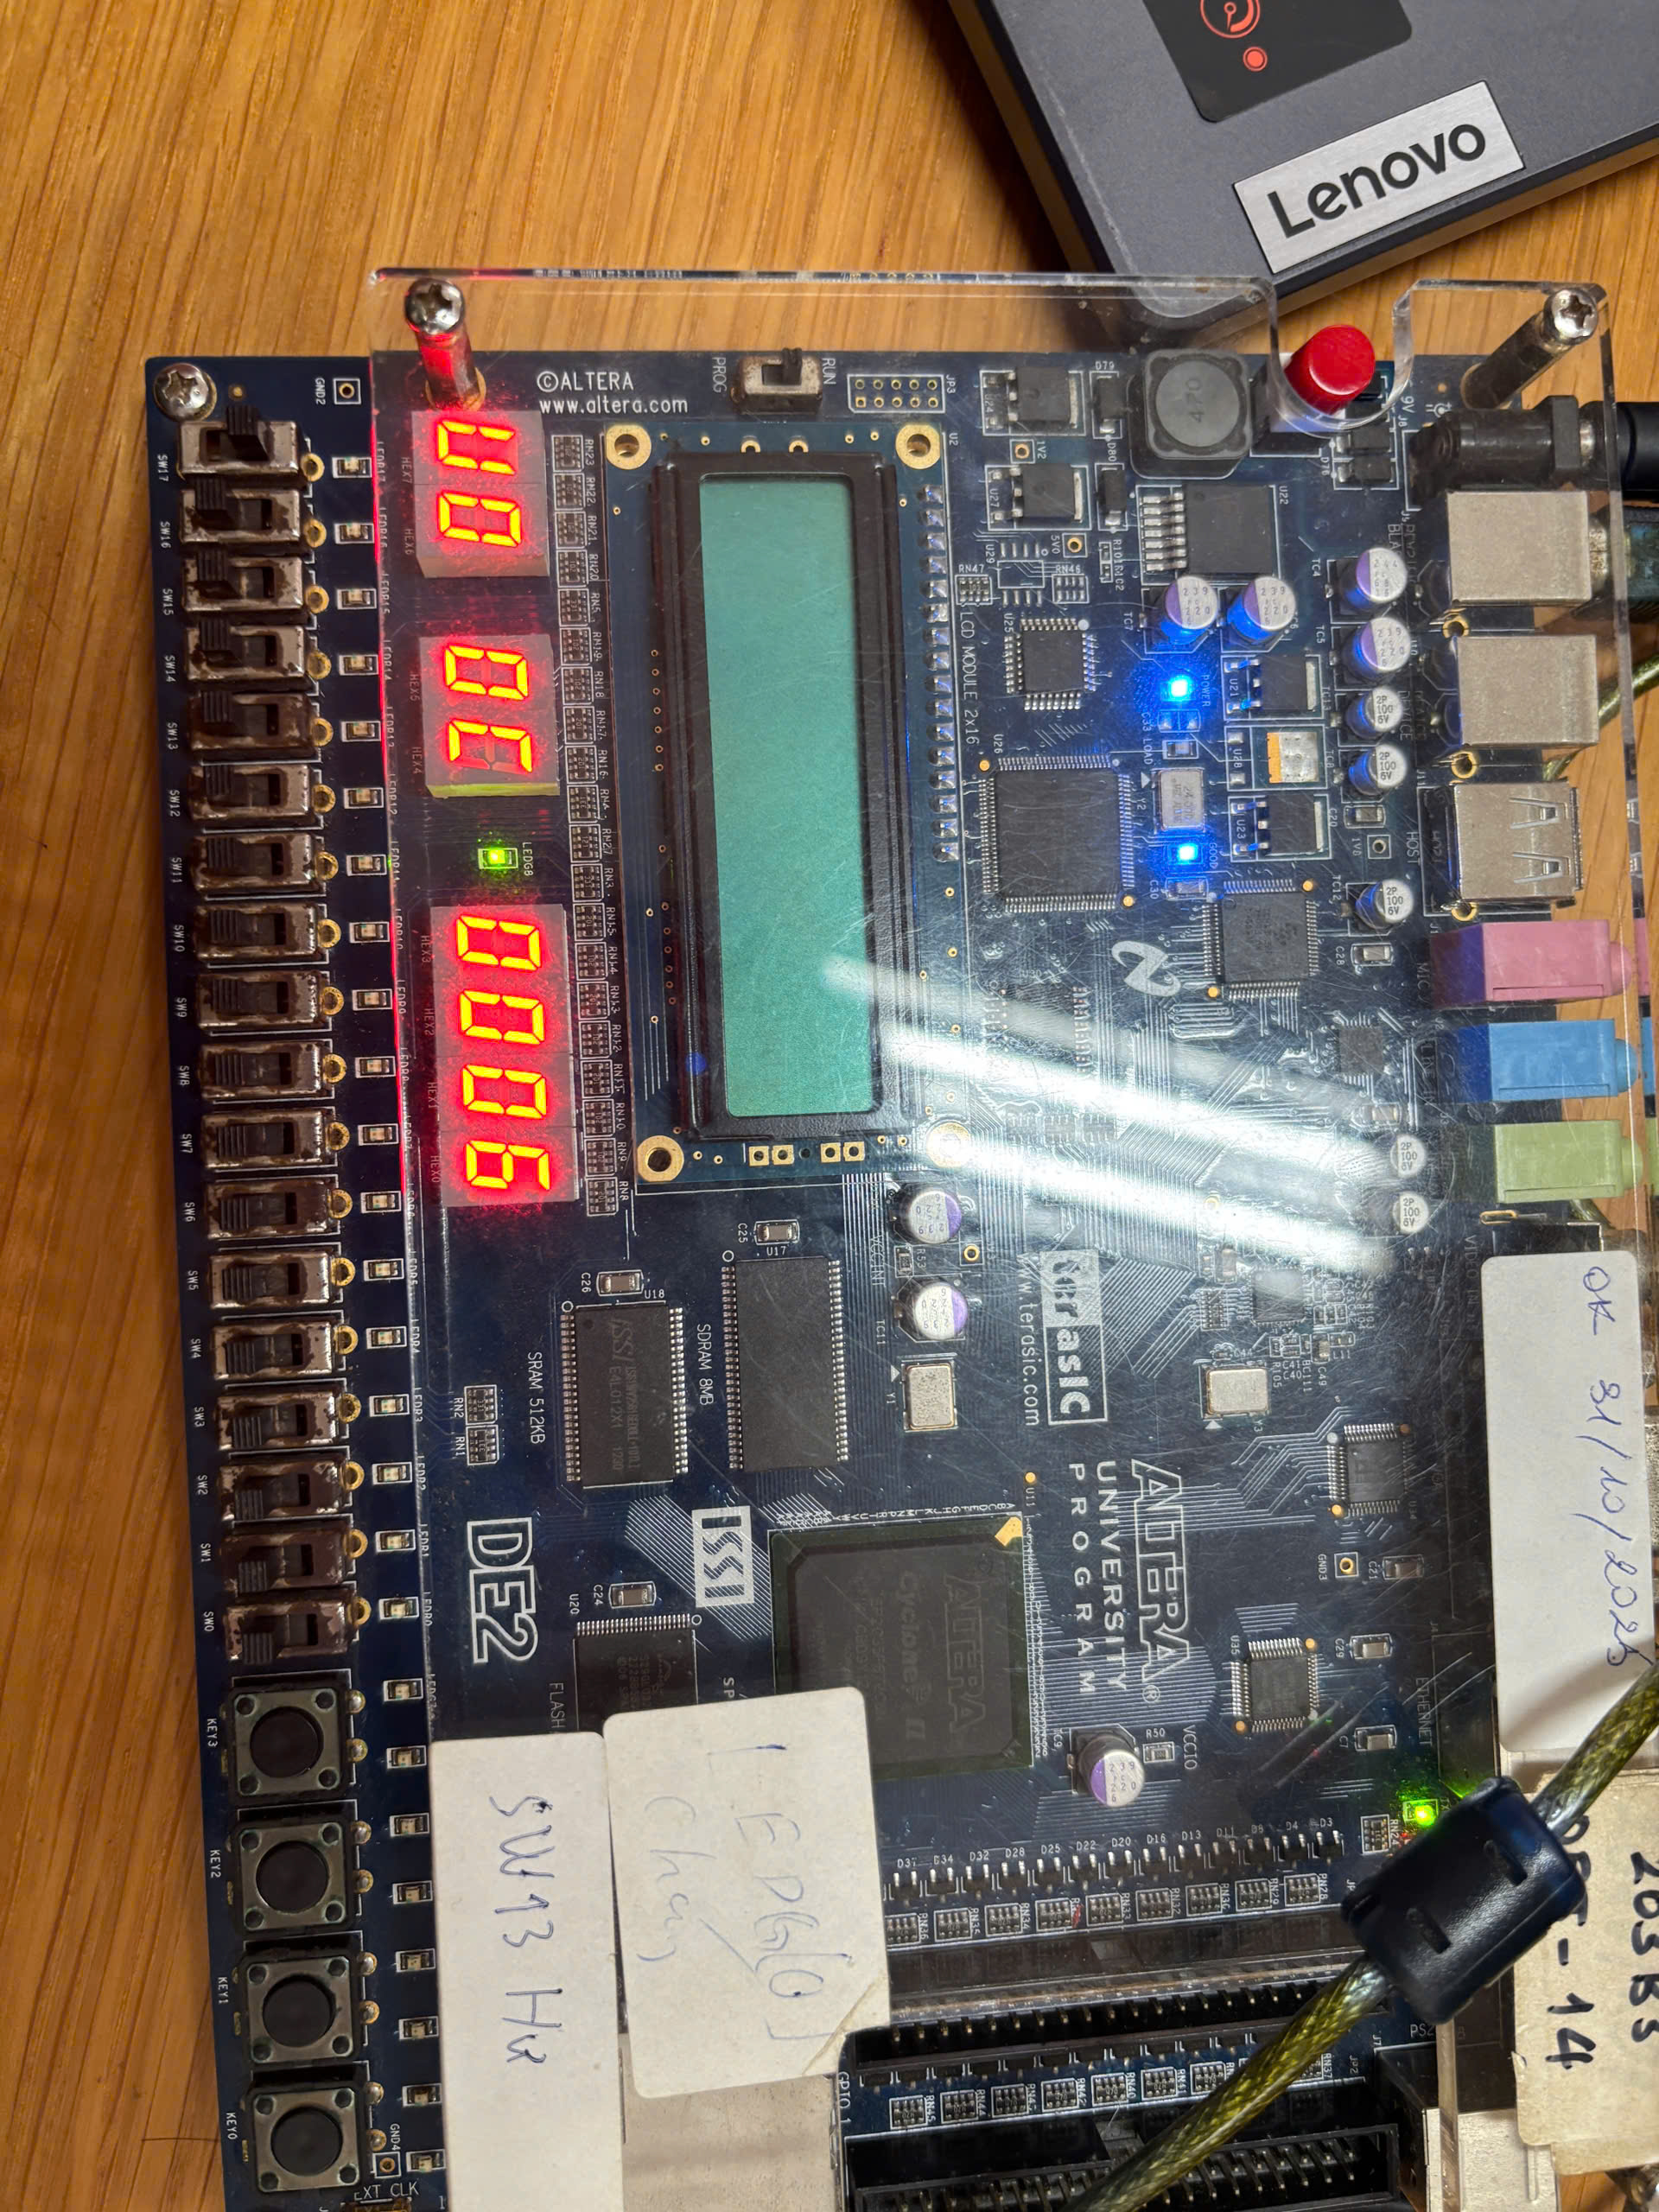
\includegraphics[width=0.7\linewidth]{figures_tech/stop_watch.jpg} 
	\caption{Stopwatch Paused via Switch 0}
\end{figure}

This application implements a digital stopwatch capable of counting from 000 to 999 on the 7-segment LED displays. It incorporates a software-based delay loop for timing and uses a physical switch to pause the counting process. The operational flow consists of the following key stages:

\begin{enumerate}
	\item \textbf{Initialization and Blanking:} The program first establishes the base addresses for the Switches (\texttt{0x10010000}) and the two HEX display clusters (\texttt{0x10002000} for HEX 3-0, \texttt{0x10003000} for HEX 7-4). It resets all 8 HEX displays to show '0' by writing the 7-segment control code \texttt{0xC0} to their respective addresses. Four independent registers (\texttt{x12} to \texttt{x15}) are initialized as decimal counters (0-9) for each digit.
	\item \textbf{State Polling (Pause Feature):} At the beginning of the main loop, the processor polls the state of the Switches. If Switch 0 (SW0) is toggled on (logic 1), the program jumps directly to the display routine, effectively skipping the increment step and pausing the stopwatch.
	\item \textbf{Ripple Carry Counting:} If not paused, the algorithm checks if the target value (1000) has been reached. If so, it resets all counters to 0. Otherwise, it increments the units counter (\texttt{x12}). If the units counter reaches 10, it is reset to 0 and a carry is passed to increment the tens counter (\texttt{x13}). This cascading logic continues up to the thousands counter (\texttt{x15}).
	\item \textbf{Decoding and Display Output:} The value of each counter register is passed to the \texttt{BCD\_TO\_HEX} subroutine. This function translates the decimal digit (0-9) into its active-low 7-segment hexadecimal representation (e.g., \texttt{0xC0} for '0', \texttt{0xF9} for '1'). The resulting codes are then stored back to the peripheral memory at the offset addresses of HEX 0 to 3 to update the physical display.
	\item \textbf{Software Delay:} Finally, the algorithm jumps to the \texttt{DELAY\_n\_100ms} subroutine, executing empty nested loops to stall the CPU for approximately 0.5 seconds. After the delay, the program branches back to the main loop to read the switch state and begin the next cycle.
\end{enumerate}
\newpage
% ---------------------------------------------------------
% QUARTUS
% ---------------------------------------------------------
\section{Quartus Compilation Report}

The project was synthesized and compiled targeting the Altera DE2 hardware board, utilizing a \textbf{Cyclone II} FPGA chip with the specific device code \textbf{EP2C35F672C6}. 

Below is a detailed summary table of the resource utilization and performance metrics extracted from the Quartus compilation report:

\begin{table}[H]
	\centering
	\renewcommand{\arraystretch}{1.2} % Increases row height for better readability
	\begin{tabular}{llc}
		\toprule
		\textbf{Metric} & \textbf{Value (Used / Total)} & \textbf{Percentage} \\ \midrule
		FPGA Device & Cyclone II EP2C35F672C6 & - \\ 
		Maximum Frequency (Slow Model) & 31.43 MHz & - \\ 
		Total logic elements & 13,866 / 33,216 & 42\% \\ 
		$\quad \hookrightarrow$ Total combinational functions & 10,898 / 33,216 & 33\% \\
		$\quad \hookrightarrow$ Dedicated logic registers & 5,305 / 33,216 & 16\% \\
		Total registers & 5,305 & - \\ 
		Total pins & 219 / 475 & 46\% \\ 
		Total memory bits & 0 / 483,840 & 0\% \\ 
		Total PLLs & 0 / 4 & 0\% \\
		\bottomrule
	\end{tabular}
	\caption{Resource Utilization and Performance Summary}
\end{table}
\newpage
% ---------------------------------------------------------
% REFERENCES
% ---------------------------------------------------------

\begin{thebibliography}{9}
	
	\bibitem{patterson}
	D.~A. Patterson and J.~L. Hennessy, \emph{Computer Organization and Design RISC-V Edition: The Hardware Software Interface}. Morgan Kaufmann.
	
	\bibitem{brown}
	S.~Brown and Z.~Vranesic, \emph{Fundamentals of Digital Logic with Verilog Design}, 3rd~ed. McGraw-Hill.
	
	\bibitem{mano_digital}
	M.~M. Mano and M.~D. Ciletti, \emph{Digital Design: With an Introduction to the Verilog HDL, VHDL, and SystemVerilog}. Pearson.
	
	\bibitem{mano_logic}
	M.~M. Mano, C.~R. Kime, and T.~Martin, \emph{Logic and Computer Design Fundamentals}, 5th~ed. Pearson, 2015.
	
	\bibitem{intro_synthesis}
	\emph{Introduction to Logic Synthesis using Verilog HDL}.
	
	\bibitem{cao_milestone}
	H.~Cao, ``Milestone 2: Computer Architecture - Design of a Single Cycle RISC-V Processor,'' rev. 2.0.0.
	
\end{thebibliography}
\newpage 
\section{Appendix}


\subsection{Hardware Implementation Video}
The following link provides a video demonstration of the program executing on the FPGA kit. You can access the video by clicking the link or scanning the QR code below:

\begin{center}
	% Clickable link
	\href{https://drive.google.com/drive/u/3/folders/1d-ZMj_vs8g-kHeXnu3KJcHw9mhhGdeYM}{Click here to view the Implementation Video (Google Drive)}
	
	\vspace{0.5cm}
	% QR Code
	\qrcode[height=2cm]{https://drive.google.com/drive/u/3/folders/1d-ZMj_vs8g-kHeXnu3KJcHw9mhhGdeYM}
\end{center}

\subsection{Application 1: Stopwatch on 7-Segment LEDs}

This application implements a digital stopwatch capable of counting from 000 to 999 on the 7-segment LED displays.

\begin{lstlisting}[style=verilog-style]
	# ==========================================
	# FILE 1: stopwatch.s
	# ==========================================
	.text
	.globl _start
	
	_start:
	# --- THIET LAP DIA CHI THEO MAPPING MOI (MILESTONE 2 SPEC) ---
	li      x23, 0x10010000    # Dia chi SWITCH
	li      x21, 0x10002000    # Dia chi LED HEX 3-0
	li      x24, 0x10003000    # Dia chi LED HEX 7-4
	
	# Reset tat ca cac den ve 0 ban dau
	li      x22, 0xC0          # Ma 7 doan cho so 0
	sb      x22, 0(x21)        # HEX0 = 0
	sb      x22, 1(x21)        # HEX1 = 0
	sb      x22, 2(x21)        # HEX2 = 0
	sb      x22, 3(x21)        # HEX3 = 0
	sb      x22, 0(x24)        # HEX4 = 0 (Ghi vao byte 0 cua 0x10003000)
	sb      x22, 1(x24)        # HEX5 = 0
	sb      x22, 2(x24)        # HEX6 = 0
	sb      x22, 3(x24)        # HEX7 = 0
	
	# Khoi tao cac bien dem
	li      x12, 0             # HEX0 = 0
	li      x13, 0             # HEX1 = 0
	li      x14, 0             # HEX2 = 0
	li      x15, 0             # HEX3 = 0
	li      x20, 10            # Gioi han dem decimal (0-9)
	li      x4 , 0x10010000    # Dia chi doc SWITCH
	
	MAIN_LOOP:
	# Kiem tra trang thai va gioi han
	li      x30, 0x01          # So sanh voi 1
	lw      x5, 0(x4)          # Doc gia tri switch
	beq     x5, x30, DISPLAY   # Neu bat SW0 thi nhay den DISPLAY (tam dung)
	beq     x15, x30, CHECK_1000 # Neu HEX3 = 1, kiem tra cac chu so con lai
	j       COUNT              # Neu chua dat, tiep tuc dem
	
	CHECK_1000:
	bne     x14, x0, COUNT
	bne     x13, x0, COUNT
	bne     x12, x0, COUNT
	j       RESET              # Reset ve 0 neu dat 1000
	
	COUNT:
	# Tang HEX0
	addi    x12, x12, 1        # HEX0 + 1
	blt     x12, x20, DISPLAY  # Neu < 10, hien thi
	
	# Reset HEX0, tang HEX1
	li      x12, 0              
	addi    x13, x13, 1
	blt     x13, x20, DISPLAY
	
	# Reset HEX1, tang HEX2
	li      x13, 0
	addi    x14, x14, 1
	blt     x14, x20, DISPLAY
	
	# Reset HEX2, tang HEX3
	li      x14, 0
	addi    x15, x15, 1
	blt     x15, x20, DISPLAY
	
	RESET:
	li      x12, 0             # Reset tat ca ve 0
	li      x13, 0
	li      x14, 0
	li      x15, 0
	
	DISPLAY:
	# Chuyen doi va hien thi HEX0
	add     x16, x0, x12       # Copy gia tri can chuyen doi
	jal     x1, BCD_TO_HEX     # Chuyen sang ma 7 doan
	sb      x22, 0(x21)        # Hien thi HEX0
	
	# Chuyen doi va hien thi HEX1
	add     x16, x0, x13
	jal     x1, BCD_TO_HEX
	sb      x22, 1(x21)
	
	# Chuyen doi va hien thi HEX2
	add     x16, x0, x14
	jal     x1, BCD_TO_HEX
	sb      x22, 2(x21)
	
	# Chuyen doi va hien thi HEX3
	add     x16, x0, x15
	jal     x1, BCD_TO_HEX
	sb      x22, 3(x21)
	
	# Delay 0.5s
	li      x29, 5             # 5 * 100ms = 0.5s
	jal     x1, DELAY_n_100ms
	
	j       MAIN_LOOP          # Lap lai
	
	# ==============================================================================
	# HAM: Chuyen doi BCD sang ma 7 doan
	# ==============================================================================
	BCD_TO_HEX:
	# Input: x16 (so BCD)
	# Output: x22 (ma 7 doan)
	ZERO:
	li      x30, 0
	bne     x16, x30, ONE
	li      x22, 0xC0      # Ma cho so 0
	ret
	ONE:
	li      x30, 1
	bne     x16, x30, TWO
	li      x22, 0xF9      # Ma cho so 1
	ret
	TWO:
	li      x30, 2
	bne     x16, x30, THREE
	li      x22, 0xA4      # Ma cho so 2
	ret
	THREE:
	li      x30, 3
	bne     x16, x30, FOUR
	li      x22, 0xB0      # Ma cho so 3
	ret
	FOUR:
	li      x30, 4
	bne     x16, x30, FIVE
	li      x22, 0x99      # Ma cho so 4
	ret
	FIVE:
	li      x30, 5
	bne     x16, x30, SIX
	li      x22, 0x92      # Ma cho so 5
	ret
	SIX:
	li      x30, 6
	bne     x16, x30, SEVEN
	li      x22, 0x82      # Ma cho so 6
	ret
	SEVEN:
	li      x30, 7
	bne     x16, x30, EIGHT
	li      x22, 0xF8      # Ma cho so 7
	ret
	EIGHT:
	li      x30, 8
	bne     x16, x30, NINE
	li      x22, 0x80      # Ma cho so 8
	ret
	NINE:
	li      x22, 0x90      # Ma cho so 9
	ret
	
	# ==============================================================================
	# HAM: Delay
	# ==============================================================================
	DELAY_n_100ms:
	# Input: x29 (so lan delay 100ms)
	DELAY_100ms:
	li      x31, 100000    # 100,000 cycles o 1MHz = 100ms
	LOOP_DELAY:
	addi    x31, x31, -1
	beq     x31, x0, NEXT_DELAY
	j       LOOP_DELAY
	NEXT_DELAY:
	addi    x29, x29, -1
	bgt     x29, x0, DELAY_100ms
	ret
\end{lstlisting}

\newpage
\subsection{Application 2: Displaying Switch Value on 7-Segment LED (SW to HEX)}

This assembly program reads the status from the Switches, extracts the decimal digits, and decodes the values for display on the HEX (7-segment) LEDs.

\begin{lstlisting}[style=verilog-style]
	# ==========================================
	# FILE 2: sw_to_hex.s
	# ==========================================
	.text
	.globl _start
	
	_start:
	# ==============================================================================
	# PHAN 1: KHOI TAO DIA CHI NGOAI VI
	# ==============================================================================
	lui     t0, 0x10010       # t0 (x5)  = 0x10010000 (Dia chi co so cua Switches)
	lui     t1, 0x10002       # t1 (x6)  = 0x10002000 (Dia chi co so cua LED HEX 3-0)
	lui     t2, 0x10003       # t2 (x7)  = 0x10003000 (Dia chi co so cua LED HEX 7-4)
	
	MAIN_LOOP:
	# ==============================================================================
	# PHAN 2: DOC DU LIEU TU SWITCH & LOC LAY 13 BIT
	# ==============================================================================
	lw      a0, 0(t0)         # a0 (x10) = Doc trang thai hien tai cua cac cong tac
	lui     t5, 0x2           # t5 (x30) = 0x00002000
	addi    t5, t5, -1        # t5 = 0x1FFF (Mat na 13 bit, gia tri max la 8191)
	and     a0, a0, t5        # a0 &= 0x1FFF (Chi lay 13 cong tac dau tien)
	
	# ==============================================================================
	# PHAN 3: TACH TUNG CHU SO THAP PHAN (CHIA LIEN TUC CHO 10)
	# ==============================================================================
	# Tach hang don vi (Digit 0)
	add     a1, a0, zero      # a1 = a0 (Nap gia tri vao doi so cua ham)
	jal     ra, DIV10_MOD10   # Goi ham chia 10. (Thuong so: a2, Phan du: a3)
	add     s0, a3, zero      # s0 (x8) = Phan du (Chu so hang don vi)
	
	# Tach hang chuc (Digit 1)
	add     a1, a2, zero      # Lay thuong so buoc truoc lam so bi chia moi
	jal     ra, DIV10_MOD10
	add     s1, a3, zero      # s1 (x9) = Chu so hang chuc
	
	# Tach hang tram (Digit 2)
	add     a1, a2, zero
	jal     ra, DIV10_MOD10
	add     s2, a3, zero      # s2 (x18) = Chu so hang tram
	
	# Tach hang ngan (Digit 3)
	add     a1, a2, zero
	jal     ra, DIV10_MOD10
	add     s3, a3, zero      # s3 (x19) = Chu so hang ngan
	
	# Tach hang chuc ngan (Digit 4)
	add     a1, a2, zero
	jal     ra, DIV10_MOD10
	add     s4, a3, zero      # s4 (x20) = Chu so hang chuc ngan
	
	# Tach hang tram ngan (Digit 5)
	add     a1, a2, zero
	jal     ra, DIV10_MOD10
	add     s5, a3, zero      # s5 (x21) = Chu so hang tram ngan
	
	# ==============================================================================
	# PHAN 4: GIAI MA VA XUAT RA LED 7 DOAN
	# ==============================================================================
	add     t3, s0, zero      # Dua hang don vi vao t3 (x28) de giai ma
	jal     ra, HEX_DECODE    # Goi ham giai ma LED (Ket qua tra ve o t6/x31)
	sb      t6, 0(t1)         # Hien thi len HEX0
	
	add     t3, s1, zero
	jal     ra, HEX_DECODE
	sb      t6, 1(t1)         # Hien thi len HEX1
	
	add     t3, s2, zero
	jal     ra, HEX_DECODE
	sb      t6, 2(t1)         # Hien thi len HEX2
	
	add     t3, s3, zero
	jal     ra, HEX_DECODE
	sb      t6, 3(t1)         # Hien thi len HEX3
	
	add     t3, s4, zero
	jal     ra, HEX_DECODE
	sb      t6, 0(t2)         # Hien thi len HEX4
	
	add     t3, s5, zero
	jal     ra, HEX_DECODE
	sb      t6, 1(t2)         # Hien thi len HEX5
	
	# Ghi so '0' co dinh vao 2 LED cao nhat
	addi    t4, zero, 0x40    # t4 = 0x40 (Ma 7 bit cua so '0')
	sb      t4, 2(t2)         # Ghi '0' ra HEX6
	sb      t4, 3(t2)         # Ghi '0' ra HEX7
	
	jal     zero, MAIN_LOOP   # Lap lai toan bo qua trinh lien tuc
	
	# ==============================================================================
	# CHUONG TRINH CON: DIV10_MOD10 (Phep chia va lay du cho 10)
	# ==============================================================================
	# Dau vao: a1 (So bi chia)
	# Dau ra:  a2 (Thuong so), a3 (Phan du)
	DIV10_MOD10:
	add     a2, zero, zero    # a2 (Quotient) = 0
	add     a3, a1, zero      # a3 (Remainder) = a1
	addi    t4, zero, 10      # t4 = 10 (So chia)
	div_loop:
	slt     t5, a3, t4        # Neu phan du < 10, t5 = 1, nguoc lai t5 = 0
	bne     t5, zero, div_end # Neu phan du < 10, thoat khoi vong lap tru
	addi    a2, a2, 1         # Tang thuong so them 1
	addi    a3, a3, -10       # Tru phan du di 10
	jal     zero, div_loop    # Tiep tuc vong lap
	div_end:
	jalr    zero, ra, 0       # Quay lai noi goi ham
	
	# ==============================================================================
	# CHUONG TRINH CON: HEX_DECODE (Giai ma so thap phan sang ma LED 7 doan)
	# ==============================================================================
	# Dau vao: t3 (x28) - Chu so tu 0 den 9
	# Dau ra:  t6 (x31) - Ma thap luc phan cua LED 7 doan tuong ung
	HEX_DECODE:
	beq     t3, zero, ret_0
	addi    t4, zero, 1
	beq     t3, t4, ret_1
	addi    t4, zero, 2
	beq     t3, t4, ret_2
	addi    t4, zero, 3
	beq     t3, t4, ret_3
	addi    t4, zero, 4
	beq     t3, t4, ret_4
	addi    t4, zero, 5
	beq     t3, t4, ret_5
	addi    t4, zero, 6
	beq     t3, t4, ret_6
	addi    t4, zero, 7
	beq     t3, t4, ret_7
	addi    t4, zero, 8
	beq     t3, t4, ret_8
	# Default (Truong hop so 9)
	addi    t6, zero, 0x10    # Ma LED cho so '9'
	jalr    zero, ra, 0       # Quay lai
	
	ret_0:  addi t6, zero, 0x40; jalr zero, ra, 0
	ret_1:  addi t6, zero, 0x79; jalr zero, ra, 0
	ret_2:  addi t6, zero, 0x24; jalr zero, ra, 0
	ret_3:  addi t6, zero, 0x30; jalr zero, ra, 0
	ret_4:  addi t6, zero, 0x19; jalr zero, ra, 0
	ret_5:  addi t6, zero, 0x12; jalr zero, ra, 0
	ret_6:  addi t6, zero, 0x02; jalr zero, ra, 0
	ret_7:  addi t6, zero, 0x78; jalr zero, ra, 0
	ret_8:  addi t6, zero, 0x00; jalr zero, ra, 0
\end{lstlisting}

\newpage
\subsection{Application 3: Single LED Control via Switch (SW to LEDR)}

This module continuously reads the input switches and drives the Red LED (LEDR) outputs directly.

\begin{lstlisting}[style=verilog-style]
	# ==========================================
	# FILE 3: sw_to_ledr.s
	# ==========================================
	.text
	.globl _start
	
	_start:
	lui     x31, 0x10000      # x31 = 0x10000000 (Dia chi co so LEDR)
	lui     x30, 0x10010      # x30 = 0x10010000 (Dia chi co so SWITCH)
	
	loop:
	lw      x9, 0(x30)        # Doc gia tri tu dia chi x30 luu vao x9
	sw      x9, 0(x31)        # Ghi gia tri tu x9 ra dia chi x31
	jal     x0, -8            # Nhay lui lai 8 byte (tuong duong 2 lenh), quay lai nhan 'loop'
\end{lstlisting}


